%\documentclass[12pt]{article}
\documentclass{pnastwo}

%\def\E {\mbox{E}}
%\def\ex {\mbox{e}}
%\def\partiald {\mbox{d}}
%\def\V {\mbox{Var}}
%\def\C {\mbox{Cov}}
%\def\se {\sigma_{\eps}}
%\def\half {\textstyle\frac{1}{2}}
%\def\quart {\textstyle\frac{1}{4}}
%\def\eight {\textstyle\frac{1}{8}}
%\def\sqrttwo {\textstyle\frac{1}{\sqrt{2}}}
%\newcommand{\eps}{\mbox{\large $\varepsilon$}}
%\newcommand{\ah}{\makebox[0pt][l]{$^a$}}
%\renewcommand{\baselinestretch}{1.325}
%\parskip 6pt plus 3pt minus 2pt
%%\special{papersize=8.25in,11.5in}
%\pagestyle{plain}
%\oddsidemargin 0pt
%\evensidemargin 0pt
%\textwidth 6.5in
%\textheight 9.1in

% Including line numbers
%\usepackage{lineno} 

% Including pdf figures
\usepackage{graphicx}

% Including math features
\usepackage{amsmath}
\usepackage{amssymb}
\usepackage{amsfonts}
\usepackage{graphicx}

% Bibliographies
\usepackage[]{natbib}
\bibpunct{(}{)}{,}{a}{}{;} 

% Including male & female symbols
\usepackage{wasysym}

\usepackage{xr}
\externaldocument{SexChromosomes_PNAS}

%\usepackage{cite}
%\usepackage[round]{natbib}
%\usepackage{/Users/otto/Library/TeXmenu/amnat} 
%\bibliographystyle{cbe}

\usepackage{color} 
\newcommand{\red}[1]{\textcolor{red}{#1}}
\newcommand{\green}[1]{\textcolor{green}{#1}}
\newcommand{\blue}[1]{\textcolor{blue}{#1}}

% Formats equations as (#)
% \renewcommand{\eqref}[1]{\textup{{\normalfont(\ref{#1}}\normalfont)}}

% Formats equations as bold #
\renewcommand{\eqref}[1]{\textup{\bf{\ref{#1}}}}

%%% font setup in order to make the article printable
%\usepackage{mathptmx}
%\usepackage{helvet}
%\renewcommand\bibfont{\fontsize{6pt}{9pt}\bfseries\sffamily}
%\renewcommand{\bibitfont}{\bibfont\slshape}
%\renewcommand{\bibbffont}{\bibfont}
%%%

\renewcommand{\bibitfont}{\fontsize{6pt}{9pt} \bibfont\slshape}

%------------------------------------------------
% DO NOT EDIT THIS SECTION
%------------------------------------------------

%% For PNAS Only:
\url{www.pnas.org/cgi/doi/10.1073/pnas.0709640104}
\copyrightyear{2008}
\issuedate{Issue Date}
\volume{Volume}
\issuenumber{Issue Number}

%----------------------------------------------------------------------------------------

\begin{document}


\markright{Recombination evolution \hspace{2.3in} Scott \& Otto}
\section{Recursion Equations}
\label{app:recurs}
% Starts equation numbers from 0 again and adds S to tag
\setcounter{equation}{0}
\renewcommand{\theequation}{S.\arabic{equation}}
\renewcommand{\thefigure}{S.\arabic{figure}}
\renewcommand{\thetable}{S.\arabic{table}}


In each generation we census the genotype frequencies in male and female haploids before haploid selection, e.g., sperm/pollen and eggs/ovules. Before haploid selection, the frequency of X-bearing male and female haploids are given by $X_{i}^{m}$ and $X_{i}^{f}$ and the frequency of Y-bearing haploids is given by $Y_{i}^{m}$ where the index $i$ specifies genotypes $MA$, $Ma$, $mA$, and $ma$. 
Selection then occurs among male haploids according to the \textbf{A} locus allele, $k$, carried by individuals with genotype $i$.
Assuming that the fraction of X-bearing haploids produced by males is $f$, the genotype frequencies after haploid selection are $X_{i}^{m,s}=f w_{k}X_{i}^{m}/\bar{w}_{H}$ and $Y_{i}^{m,s}=(1-f) w_{k}Y_{i}^{m}/\bar{w}_{H}$, where $\bar{w}_{H}=\sum_{i=1}^{4}f w_{k}X_{i}^{m}+(1-f)w_{k}Y_{i}^{m}$ is the mean fitness of male haploids. Random mating then occurs between gametes to produce diploid females with genotype $ij$ at frequency $x_{ij}=X_{i}^{f}X_{j}^{m,s}$ and diploid males at frequency $y_{ij}=X_{i}^{f}Y_{j}^{m,s}$. 
In females, individuals with genotype $ij$ are equivalent to those with genotype $ji$. 
For simplicity we denote the frequency of genotype $ij$ in females to the average of these frequencies, $x_{ij}=(X_{i}^{f}X_{j}^{m,s}+X_{j}^{f}X_{i}^{m,s})/2$.
Note that the sex ratio before diploid selection depends both on the production of X-bearing haploids by fathers ($f$) and on haploid selection ($w_{k}$).
However, $f$ does not enter into any results, indicating that the main force driving recombination evolution is not to balance the current sex ratio. 

\begin{table}[ht]
\centering
\smallskip
\caption{Fitness of different genotypes.}
\begin{tabular}{l c c c c c}
\hline\hline
  Genotype & $A$ & $a$ & $AA$ & $Aa$ & $aa$ \\ [0.5ex] \hline
  Fitness in males & $w_{A}$ & $w_{a}$ & $w_{AA}^{m}$ & $w_{Aa}^{m}$ & $w_{aa}^{m}$ \\
  Fitness in females & 1 & 1 & $w_{AA}^{f}$ & $w_{Aa}^{f}$ & $w_{aa}^{f}$\\
  \hline \hline
  \label{tab:fitnesstable}
 \end{tabular}
\end{table}

\begin{table}[ht]
\centering
\smallskip
\caption{Marginal fitnesses of Y$\mathbf{A}$ and X$\mathbf{a}$ haplotypes}
\begin{tabular}{l l}
\hline\hline
  $\bar{w}_{YA}^{m}$ & $=(w_{A}(p_{Xf}w_{AA}^f+(1-p_{Xf}) w_{Aa}^f))$ \\
  $\bar{w}_{Xa}^{mat,m}$ & $=p_{Ym}w_{A}w_{Aa}^m+(1-p_{Ym})w_{a}w_{aa}^m$ \\
  $\bar{w}_{Xa}^{pat,f}$ & $=p_{Xf}w_{a}w_{Aa}^f+(1-p_{Xf})w_{a}w_{aa}^f$ \\
  $\bar{w}_{Xa}^{mat,f}$ & $=p_{Xm}w_{A}w_{Aa}^f+(1-p_{Xm})w_{a}w_{aa}^f$\\
  \hline \hline
  \label{tab:marginalFitnesses}
 \end{tabular}
\end{table}


Selection among diploids then occurs according to the diploid genotype at the \textbf{A} locus, $k$, for an individual of type $ij$ (see Table \ref{tab:fitnesstable}). The diploid frequencies after selection are given by $x_{ij}^{s}=w_{k}^{f} x_{ij}/\bar{w}^{f}$ in females and $y_{ij}^{s}=w_{k}^{m}  y_{ij}/\bar{w}^{m}$ in males, where $\bar{w}^{f}= \sum_{i=1}^{4}\sum_{j=1}^{4}w_{k}^{f}x_{ij}$ and $\bar{w}^{m}= \sum_{i=1}^{4}\sum_{j=1}^{4}w_{k}^{m}y_{ij}$ are the mean fitnesses of females and males, respectively. 
Finally, these diploids undergo meiosis to produce the next generation. The haplotype frequencies in the next generation of eggs/ovules is given by:

\begin{subequations}
\begin{equation}
X_{MA}^{f'}=\left( \sum_{j=1}^{4} x_{1j}^{s} \right) - R_{f}(x_{14}^{s}-x_{23}^{s})
\end{equation}
\begin{equation}
X_{Ma}^{f'}=\left( \sum_{j=1}^{4} x_{2j}^{s} \right) + R_{f}(x_{14}^{s}-x_{23}^{s})
\end{equation}
\begin{equation}
X_{mA}^{f'}=\left( \sum_{j=1}^{4} x_{3j}^{s} \right) + R_{f}(x_{14}^{s}-x_{23}^{s})
\end{equation}
\begin{equation}
X_{ma}^{f'}=\left( \sum_{j=1}^{4} x_{4j}^{s} \right) - R_{f}(x_{14}^{s}-x_{23}^{s})
\end{equation}
\label{eq:recXf}
\end{subequations}

\noindent
which only involve the recombination rate between the \textbf{A} locus and the \textbf{M} locus in females ($R_{f}$). 
In males, recombination between the SDR and the \textbf{A} locus or the \textbf{M} also affects the frequencies of haplotypes produced. 
The frequency of haplotypes among X-bearing sperm/pollen (before haploid selection) in the next generation are given by

\begin{subequations}
\begin{equation}
\begin{split}
X_{MA}^{m'}=&\left( \sum_{j=1}^{4} y_{1j}^{s} \right) - r_{MM}(y_{12}^{s}-y_{21}^{s})\\
&- (R_{m}+r_{Mm}-2\chi)(y_{13}^{s}-y_{31}^{s})-(R_{m}+r_{Mm}-\chi)y_{14}^{s}\\
&+(r_{Mm}-\chi)y_{41}^{s}+\chi \ y_{23}^{s}+(r_{Mm}-\chi)y_{32}^{s}
\end{split}
\end{equation}
%
\begin{equation}
\begin{split}
X_{Ma}^{m'}=&\left( \sum_{j=1}^{4} y_{2j}^{s} \right) - r_{MM}(y_{21}^{s}-y_{12}^{s})\\
&- (R_{m}+r_{Mm}-2\chi)(y_{24}^{s}-y_{42}^{s})-(R_{m}+r_{Mm}-\chi)y_{23}^{s}\\
&+(r_{Mm}-\chi)y_{32}^{s}+\chi \ y_{14}^{s}+(r_{Mm}-\chi)y_{41}^{s}
\end{split}
\end{equation}
%
\begin{equation}
\begin{split}
X_{mA}^{m'}=&\left( \sum_{j=1}^{4} y_{3j}^{s} \right) - r_{mm}(y_{34}^{s}-y_{43}^{s})\\
&- (R_{m}+r_{Mm}-2\chi)(y_{31}^{s}-y_{13}^{s})-(R_{m}+r_{Mm}-\chi)y_{32}^{s}\\
&+(r_{Mm}-\chi)y_{23}^{s}+\chi \ y_{41}^{s}+(r_{Mm}-\chi)y_{14}^{s}
\end{split}
\end{equation}
%
\begin{equation}
\begin{split}
X_{ma}^{m'}=&\left( \sum_{j=1}^{4} y_{4j}^{s} \right) - r_{mm}(y_{43}^{s}-y_{34}^{s})\\
&- (R_{m}+r_{Mm}-2\chi)(y_{42}^{s}-y_{24}^{s})-(R_{m}+r_{Mm}-\chi)y_{41}^{s}\\
&+(r_{Mm}-\chi)y_{14}^{s}+\chi \ y_{32}^{s}+(r_{Mm}-\chi)y_{23}^{s}
\end{split}
\end{equation}
\label{eq:recXm}
\end{subequations}

\noindent
and the frequencies of Y-bearing sperm/pollen haplotypes (before haploid selection) are given by

\begin{subequations}
\begin{equation}
\begin{split}
Y_{MA}^{m'}=&\left( \sum_{j=1}^{4} y_{1j}^{s} \right) - r_{MM}(y_{21}^{s}-y_{12}^{s})\\
&- (R_{m}+r_{Mm}-2\chi)(y_{31}^{s}-y_{13}^{s})-(R_{m}+r_{Mm}-\chi)y_{41}^{s}\\
&+(r_{Mm}-\chi)y_{14}^{s}+\chi \ y_{32}^{s}+(r_{Mm}-\chi)y_{23}^{s}
\end{split}
\end{equation}
%
\begin{equation}
\begin{split}
Y_{Ma}^{m'}=&\left( \sum_{j=1}^{4} y_{2j}^{s} \right) - r_{MM}(y_{12}^{s}-y_{21}^{s})\\
&- (R_{m}+r_{Mm}-2\chi)(y_{42}^{s}-y_{24}^{s})-(R_{m}+r_{Mm}-\chi)y_{32}^{s}\\
&+(r_{Mm}-\chi)y_{23}^{s}+\chi \ y_{41}^{s}+(r_{Mm}-\chi)y_{14}^{s}
\end{split}
\end{equation}
%
\begin{equation}
\begin{split}
Y_{mA}^{m'}=&\left( \sum_{j=1}^{4} y_{3j}^{s} \right) - r_{mm}(y_{43}^{s}-y_{34}^{s})\\
&- (R_{m}+r_{Mm}-2\chi)(y_{13}^{s}-y_{31}^{s})-(R_{m}+r_{Mm}-\chi)y_{23}^{s}\\
&+(r_{Mm}-\chi)y_{32}^{s}+\chi \ y_{14}^{s}+(r_{Mm}-\chi)y_{41}^{s}
\end{split}
\end{equation}
%
\begin{equation}
\begin{split}
Y_{ma}^{m'}=&\left( \sum_{j=1}^{4} y_{4j}^{s} \right) - r_{mm}(y_{34}^{s}-y_{43}^{s})\\
&- (R_{m}+r_{Mm}-2\chi)(y_{24}^{s}-y_{42}^{s})-(R_{m}+r_{Mm}-\chi)y_{14}^{s}\\
&+(r_{Mm}-\chi)y_{41}^{s}+\chi \ y_{23}^{s}+(r_{Mm}-\chi)y_{32}^{s}
\end{split}
\end{equation}
\label{eq:recY}
\end{subequations}

\section{Invasion of recombination modifiers}

%In the main text, we consider selected loci that are initially loosely linked to the SDR such that $\hat{p}_{Xm}=\hat{p}_{Ym}$. 
Invasion of modifiers that create a strong linkage between the X and $a$ allele is determined by the largest solution to the characteristic polynomial

\begin{equation}
\begin{split}
{\lambda_{Xa}}^2- \lambda_{Xa} \bar{w}_{Xa}^{mat,f} /\bar{w}^{f}- (\bar{w}_{Xa}^{pat,f}/\bar{w}^{f})(\bar{w}_{Xa}^{mat,m}/\bar{w}^{m})=0
.
\end{split}
\label{eq:Xcharpoly}
\end{equation}

\noindent
This can be solved for $\lambda_{Xa}$ if we assume that the selected locus is initially loosely linked to the SDR ($r_{MM}$) and that there are no sex differences in selection ($w_{ij}^m=w_{ij}^f=w_{ij}$). 
The equilibrium frequency of the $A$ allele when maintained at a polymorphic equilibrium by selection is then

\begin{equation}
\hat{p}_{Xm}=\hat{p}_{Ym}=\hat{p}_{Xf}=
\frac{2 w_{a} w_{aa}- w_{Aa}(w_{A}+w_{a})}{2\left(w_{A}(w_{AA}-w_{Aa})+w_{a}(w_{aa}-w_{Aa})\right)}
.
\label{eq:PASpolyeq}
\end{equation}

\noindent
This equilibrium is valid and stable when

\begin{equation}
\begin{split}
w_{Aa}(w_{A}+w_{a})&>2w_{A} w_{AA} \text{ and}\\
w_{Aa}(w_{A}+w_{a})&>2w_{a} w_{aa}
.
\end{split}
\label{eq:PASstability}
\end{equation}

\noindent
Therefore, a polymorphism can be maintained either if there is heterozygote advantage in diploids ($w_{Aa}>w_{aa}$ and $w_{Aa}>w_{AA}$) or if there is antagonistic selection between haploids and diploids (e.g., $w_{A}>w_{a}$ and $w_{aa}>w_{Aa}>w_{AA}$) or a combination of both \citep{Immler:2012tl}. 

After this equilibrium is reached, the invasion of a modifier that brings the $A$ allele into linkage with the Y is given by 

\begin{equation}
\lambda_{YA}=
1+
\frac{(w_{A}-w_{a})w_{Aa}(w_{A}+w_{a})(w_{Aa}(w_{A}+w_{a})-2w_{AA}w_{A})}
{(w_{A}+w_{a})({w_{Aa}}^2(w_{A}+w_{a})^2-4w_{A}w_{AA}w_{a}w_{aa})}
,
\label{eq:YinvPAS}
\end{equation}

\noindent
where $\lambda_{YA}>1$ indicates that the modifier increases in frequency. 
Given that a polymorphism at the \textbf{A} locus is initially stable (conditions \ref{eq:PASstability} are met) the sign of $\lambda_{YA}-1$ depends on the sign of $w_{A}-w_{a}$. 
That is, modifiers that bring the allele favoured in haploids (e.g., $A$ when $w_{A}>w_{a}$) into tight linkage with the Y will spread.  

Similarly, condition \eqref{eq:XAinvconds} for the invasion of modifiers that bring the $a$ allele into tight linkage with the X chromosome is satisfied if

\begin{equation}
\frac{(w_{A}-w_{a})w_{Aa}(w_{A}+w_{a})(w_{Aa}(w_{A}+w_{a})-2w_{AA}w_{A})}
{2(w_{A}+w_{a})({w_{Aa}}(w_{A}+w_{a})-w_{A}w_{AA}-w_{a}w_{aa})}>0,
\label{eq:XinvcondsPAS}
\end{equation}

\noindent
which requires $w_{A}>w_{a}$, given that conditions \eqref{eq:PASstability} are met. These results indicate that recombination modifiers invade if they bring the X into tight linkage with the allele that is less fit during haploid selection, even without the weak selection assumptions in equation \eqref{eq:XinvEquil} and without sex differences in selection in the diploid phase. 

In the main text and above, we consider the invasion of recombination suppressors that bring the $a$ allele into tight linkage with the X when the \textbf{A} locus is initially loosely linked to the SDR ($r_{MM}=1/2$) such that $\hat{p}_{Xm}=\hat{p}_{Ym}$. 
Here, we consider cases where $r_{MM}<1/2$ and define the difference in the frequency of the $A$ allele between X- and Y-bearing pollen/sperm as $\delta_{XY}=\hat{p}_{Ym}-\hat{p}_{Xm}$. 
We assume that selection is weak relative to recombination such that $\delta$, $\delta_{XY}$, and $\delta_{H}$ are all small (of order $\epsilon^2$). 
Invasion is then given by

\begin{equation}
\lambda_{Xa}' =
\lambda_{Xa}\left(1-(1-2\ r_{MM})(3+2 w_{Aa}^{f}/\bar{w}^{f})\right)
+\frac{w_{Aa}^{f}\delta_{XY}}{3\bar{w}^{f}}
\label{eq:XaprimeEq}
\end{equation}

\noindent
Under the conditions where $\lambda_{Xa}>1$, we would expect that the $a$ allele is associated with the X such that $\delta_{XY}<0$. 
Thus, \eqref{eq:XaprimeEq} indicates that selection in favour of modifiers that suppress recombination is less strong when $r_{MM}<1/2$ ($\lambda_{Xa}'<\lambda_{Xa}$), in which case intralocus conflicts are initially partially resolved by reduced recombination. 

%\newpage

\section{Invasion of Modifiers That Increase Recombination from an Initially Low Level}

%Here, we will assume that the selected locus, \textbf{A}, is between the SDR and modifier locus, \textbf{M} such that $\chi=r_{ij} R_{M}$ without interference. 
We consider a population in which linkage is tight between the \textbf{A} locus and the SDR ($r_{MM}$ is of order $\epsilon$, where the $M$ allele is initially fixed). 
%and then evaluate the spread of a rare mutant at the modifier locus that increases the recombination between \textbf{A} and the SDR by a small amount ($r_{Mm}-r_{MM}$ is of order $epsilon$). 
Recombination has no effect if the \textbf{A} locus is fixed for one allele, we therefore focus on the five equilibria that maintain both $A$ and $a$ alleles, of which four are given to leading order by:

\begin{equation*}
\begin{split}
(A)\ \ \ &\hat{p}_{Ym}=0,\ \hat{p}_{Xf}=\frac{\alpha}{\alpha+\beta},\  \hat{p}_{Xm}=\frac{w_{Aa}^{m} \alpha}{w_{Aa}^{m}\alpha+w_{aa}^{m}\beta}\\
(A')\ \ \ &\hat{p}_{Ym}=1,\ \hat{p}_{Xf}=1-\frac{\alpha'}{\alpha'+\beta'},\  \hat{p}_{Xm}=1-\frac{w_{Aa}^{m} \alpha'}{w_{Aa}^{m}\alpha'+w_{aa}^{m}\beta'}\\
(B)\ \ \ &\hat{p}_{Ym}=0,\ \hat{p}_{Xf}=1,\ \hat{p}_{Xm}=1\\
(B')\ \ \ &\hat{p}_{Ym}=1,\ \hat{p}_{Xf}=0,\ \hat{p}_{Xm}=0\\
\end{split}
\end{equation*}
\begin{equation*}
\begin{split}
\alpha=&w_{Aa}^{f} (w_{aa}^{m}w_{a}+w_{Aa}^{m}w_{A})-2w_{aa}^{f}w_{aa}^{m}w_{a}\\
\alpha '=&w_{Aa}^{f} (w_{AA}^{m}w_{A}+w_{Aa}^{m}w_{a})-2w_{AA}^{f}w_{AA}^{m}w_{A}\\
\beta=&w_{Aa}^{f} (w_{aa}^{m}w_{a}+w_{Aa}^{m}w_{A})-2w_{AA}^{f}w_{Aa}^{m}w_{A}\\
\beta '=&w_{Aa}^{f} (w_{AA}^{m}w_{A}+w_{Aa}^{m}w_{a})-2w_{aa}^{f}w_{Aa}^{m}w_{a}\\
\end{split}
\end{equation*}

\noindent
A fifth equilibrium $(C)$ also exists where $A$ is present at an intermediate frequency on the Y chromosome ($0<\hat{p}_{Y}<1$). However, equilibrium $(C)$ is never locally stable when $r_{MM} \approx 0$ and is therefore not considered further. 
Thus, the Y can either be fixed for the $a$ allele (equilibria $A$ and $B$) or the $A$ allele (equilibria $A'$ and $B'$).
The X chromosome can then either be polymorphic (equilibria $A$ and $A'$) or fixed for the alternative allele (equilibria $B$ and $B'$).
Since equilibria $(A)$ and $(B)$ are equivalent to equilibria $(A')$ and $(B')$ with the labelling of $A$ and $a$ alleles interchanged, we discuss only equilibria $(A')$ and $(B')$, in which the Y$A$ haplotype is favoured (as in the previous section), without loss of generality. 

We next calculate when $(A')$ and $(B')$ are locally stable for $r_{MM}=0$. According to the `small parameter theory' \citep{Karlin:1972ab,Karlin:1972dq}, these stability properties are unaffected by small amounts of recombination between the SDR and \textbf{A} locus, although equilibrium frequencies may be slightly altered. 
For the $A$ allele to be stably fixed on the Y requires that $\bar{w}_{YA}^{m}>\bar{w}_{Ya}^{m}$, where the marginal fitnesses of Y$A$ and Y$a$ haplotypes are $\bar{w}_{YA}^{m}$ (as above) and $\bar{w}_{Ya}^{m}=w_{Aa}^{m}p_{Xf} + w_{aa}^{m}(1-p_{Xf})$, respectively.
Substituting $\hat{p}_{Xf}$ from above, fixation of the $A$ allele on the Y requires that $\gamma_{i}>0$ where $\gamma_{(A')}=w_{A}(w_{Aa}^{m} \alpha'+w_{AA}^{m} \beta')-w_{a}(w_{aa}^{m} \alpha'+w_{Aa}^{m} \beta')$ for equilibrium $(A')$ and $\gamma_{(B')}=w_{Aa}^{m}w_{A}-w_{aa}^{m}w_{a}$ for equilibrium $(B')$.
Stability of a polymorphism on the X chromosome (equilibrium $A'$) further requires that $\alpha' >0$ and $\beta' >0$. 
Fixation of the $a$ allele on the X (equilibrium $B'$) is mutually exclusive with $(A')$ and requires that $\beta'<0$. 
We will assume that these conditions are met such that population has reached a stable equilibrium at the \textbf{A} locus when considering evolution at the modifier locus. 

To consider recombination rate evolution, we evaluate whether a mutant allele, $m$, can invade if it modifies the recombination rate between \textbf{A} and the SDR by a small amount ($|r_{mm}-r_{MM}|$ and $|r_{Mm}-r_{MM}|$ are of order $\epsilon$). 
As above, we use the leading eigenvalue, $\lambda$, from a local stability analysis to evaluate the spread of a rare mutant modifier, where now $\lambda_{i}$ determines invasion into a population at equilibrium $i$. 
Firstly, because stability of equilibrium $(A')$ requires that $\alpha '>0$ and $\beta '>0$ and all fitnesses must be non-negative, we can define the following series of $\kappa$ terms, which must be positive when $(A')$ is locally stable. 

\begin{equation*}
\begin{split}
\kappa_{1} &=w_{aa}^{f}\alpha '+w_{Aa}^{f}\beta '\\
\kappa_{2} &=w_{Aa}^{f} \alpha '+w_{AA}^{f} \beta '\\
\kappa_{3}&=w_{Aa}^{m} \alpha '+w_{AA}^{m}\beta '\\
\kappa_{4}&=w_{aa}^{f} \alpha '+w_{AA}^{f} \beta '\\
\kappa_{5}&=w_{Aa}^{m}w_{a}+w_{AA}^{m}w_{A}\\
\kappa_{6}&=w_{Aa}^{m}w_{a}w_{AA}^{m}w_{A} \\
\kappa_{7}&=w_{aa}^{f}w_{Aa}^{m}w_{a}  \alpha ' + w_{AA}^{f}w_{AA}^{m}w_{A}  \beta '\\
\kappa_{8}&=w_{aa}^{m}\alpha ' \alpha '+2w_{Aa}^{m} \alpha ' \beta '+w_{AA}^{m} \beta ' \beta '\\
\kappa_{9}&=w_{Aa}^{m}w_{a} \alpha '+w_{AA}^{m}w_{A} \beta ' \\
\kappa_{10}&=w_{Aa}^{f}\kappa_{9}+2 \kappa_{6}\kappa_{4}/\kappa_{5}
\end{split}
\end{equation*}

\noindent
These are useful in determining the magnitude of $\lambda_{(A')}$, which determines invasion of modifiers and is given by

\begin{equation}
\lambda_{(A')}=1+(r_{Mm}-r_{MM}) \frac{w_{Aa}^{m}\alpha ' K_{1}}{w_{a}R_{m}(w_{aa}^{m} \alpha '+w_{Aa}^{m} \beta ')K_{2}}
\end{equation}

\noindent
where we neglect terms of order $\epsilon^2$ and higher and $K_{2}$ is strictly positive,

\begin{equation*}
\begin{split}
K_{2}=& R_{f} 2w_{Aa}^{f}\kappa_{3}\kappa_{5} (\alpha '+\beta ')\kappa_{10}
+R_{f}R_{m} w_{Aa}^{m}w_{AA}^{m}2w_{a}w_{A}K_{3}\kappa_{3}\kappa_{4}/\kappa_{5}\\
&+ R_{m} w_{Aa}^{m}w_{AA}^{m}(1-2R_{f})\big(w_{a} \beta ' \kappa_{1}(2w_{AA}^{m}w_{A}\kappa_{2}+\kappa_{10})
+w_{A}\alpha ' \kappa_{2}(2w_{Aa}^{m}w_{a}\kappa_{1}+\kappa_{10})\big)\\
\end{split}
\end{equation*}

\noindent
such that $\lambda_{(A')}>1$ if and only if $(r_{Mm}-r_{MM})K_{1}>0$, where

\begin{equation*}
\begin{split}
K_{1}=&-(1-2R_{f})R_{m} \gamma_{(A')} \kappa_{1}\kappa_{2}\kappa_{6}-R_{m}R_{f}\gamma_{(A')} \kappa_{4} \kappa_{6} \big(\kappa_{7}/\kappa_{5} +  w_{Aa}^{f} (\alpha '+\beta ')/2\big)\\
&-R_{f}\gamma_{(A')} w_{Aa}^{f}w_{a}\kappa_{1}\kappa_{3}\kappa_{5}\\
&+R_{f} w_{Aa}^{f}w_{Aa}^{m}(\gamma_{(A')}\alpha '+R_{m}w_{a}\kappa_{8})\big( 
(w_{Aa}^{m}-w_{AA}^{m})w_{a}w_{A}  \kappa_{4}
+(w_{A}-w_{a})w_{Aa}^{f}  \kappa_{5}(\alpha '+\beta ')/2  \big)\\
%
%\frac{w_{aa}^{f} \alpha '+w_{AA}^{f} \beta '}{w_{AA}^{m} w_{A}+w_{Aa}^{m} w_{a}}\right)\\
%FAa MAa (Maa PXa +  MAa PXA) ((MAA (factorA)^2 + (2 MAa factorA + Maa factorB) factorB) 
%        (FAa factorM (PXA - PXa) + 
 %    factorI (Maa - MAa) PXa PXA) PYA)
\end{split}
\end{equation*}

\noindent
Modifiers that increase recombination ($r_{Mm}-r_{MM}>0$) therefore only spread if $K_{1}>0$. 
Only the last term of $K_{1}$ can be positive, and this term can only be positive if either $w_{Aa}^{m}>w_{AA}^{m}$ or $w_{A}>w_{a}$.
Thus, for increased recombination to be favoured by selection ($K_{1}>0$), heterozygous males must be more fit that males homozygous for the allele fixed on the Y and/or the allele fixed on the Y must be favoured during haploid selection. 
Since the $A$ allele is fixed on the Y, $w_{Aa}^{m}>w_{AA}^{m}$ implies that X chromosomes bearing the $a$ allele are favoured during selection in males. 
If a polymorphism is maintained on the X (equilibrium $A'$), counter-selection must favour the $A$ allele during haploid selection and/or selection in females when $w_{Aa}^{m}>w_{AA}^{m}$. 
In addition, when linkage between the modifier locus and the selected locus is tight (at least in females, $R_{f}=0$), $K_{1}$ is always negative and increased recombination is never favoured. 

We next consider the invasion of a recombination modifier into a population at equilibrium $(B')$. Local stability of this equilibrium requires that $(-\beta ')>0$ and $\gamma_{(B')}>0$. 
Ignoring terms of order $\epsilon^2$ and higher, 

\begin{equation*}
\lambda_{(B')}=1+ \frac{(r_{Mm}-r_{MM})K_{4}}{4(\gamma_{(B')}+R_{m}w_{aa}^{m}w_{a})((-\beta ')+w_{Aa}^{f}(R_{f}w_{Aa}^{m}w_{a}+R_{m}w_{AA}^{m}w_{A}(1-R_{f}))}
\end{equation*}

\noindent
where

\begin{equation*}
\begin{split}
K_{4}=&-2\gamma_{(B')}(-\beta ')-(2R_{f}+R_{m}(1-R_{f}))w_{Aa}^{f}w_{AA}^{m}w_{A}\gamma_{(B')}\\
&-R_{m}(-\beta ')w_{aa}^{m}w_{a}\\
&+R_{f}(w_{A}-w_{a})w_{Aa}^{f}w_{Aa}^{m}(2 \gamma_{(B')}+R_{m}w_{aa}^{m}w_{a})\\
&+R_{f}R_{m}(w_{Aa}^{m}-w_{AA}^{m})w_{Aa}^{f}w_{Aa}^{m}w_{a}w_{A}
\end{split}
\end{equation*}

\noindent
Therefore $\lambda_{(B')}>1$ if and only if $(r_{Mm}-r_{MM})K_{4}>0$. 
The only terms in $K_{4}$ that can be positive again involve the factors $(w_{A}-w_{a})$ and $(w_{Aa}^{m}-w_{AA}^{m})$, such that either $w_{Aa}^{m}>w_{AA}^{m}$ or $w_{a}>w_{A}$ are again necessary (but not sufficient) conditions for the invasion of modifiers that increase recombination. 

Finally, we re-write the condition $K_{4}>0$ to obtain

\begin{equation}
\begin{split}
w_{aa}^{f}<&w_{Aa}^{f}\left(1
-\gamma_{(B')}R_{f}(2-R_{m})R_{m})
-\gamma_{(B')}(w_{Aa}^{m}-w_{AA}^{m})K_{5}
+(w_{A}-w_{a})K_{6}\right)/K_{7}
\end{split}
\label{eq:FAAcond}
\end{equation}

\noindent
where the following terms are positive

\begin{equation*}
\begin{split}
K_{5}=&(1-R_{f})(2 \gamma_{(B')}(1-R_{m})+R_{m}w_{Aa}^{m}w_{a})/w_{Aa}^{m}\\
K_{6}=&(R_{f}R_{m}w_{A}{w_{Aa}^{m}}^2+(w_{AA}^{m}(1-R_{f})+R_{f}w_{Aa}^{m})(2 \gamma_{(B')}(1-R_{m})+w_{Aa}^{m}w_{A}R_{m}))\\
K_{7}=&4 \gamma_{(B')}+2 w_{aa}^{m}w_{a}R_{m}
\end{split}
\end{equation*}
 
\noindent
Thus, if haploid selection favours the $A$ allele, then condition \eqref{eq:FAAcond} can be met whether selection among diploid females favours allele $A$ or $a$ ($w_{aa}^{f}<w_{Aa}^{f}$ or $w_{aa}^{f}>w_{Aa}^{f}$). 
However, if haploid selection favours the $a$ allele ($w_{a}>w_{A}$), the evolution of increased recombination requires that $w_{Aa}^{m}>w_{AA}^{m}$ (see above), and equation \eqref{eq:FAAcond} shows that selection must favour the $A$ allele during selection in females ($w_{aa}^{f}<w_{Aa}^{f}$). 
Thus, increased recombination is only favoured if the $A$ allele is favoured during selection in females ($w_{aa}^{f}<w_{Aa}^{f}$) and/or the $A$ allele is favoured during haploid selection ($w_{A}>w_{a}$).
Only under these conditions is it possible for recombination between the X$A$ and Y$a$ to produce X$A$ gametes that are favoured over the short term (in daughters and/or gametes/gametophytes, respectively).

One might not expect selection to favour X$A$ haplotypes because an $A$ allele on an average X background should either have the same fitness as an $a$ allele (when a polymorphism is maintained, equilibrium $A'$) or lower fitness (when $A$ is fixed, equilibrium $B'$). 
However, an X$A$ haplotype created by recombination in males is found in a male haploid (pollen or sperm), not on an average X background (which is weighted across X-bearing male sperm/pollen and female eggs/ovules). 
Increased recombination does not evolve if $R_{f}$ and $R_{m}$ are small because the modifier remains linked to the haplotypes it creates, which will eventually be found on all backgrounds. 
However, when $R_{f}$ and $R_{m}$ are sufficiently large, modifiers that increase recombination can gain a transient fitness advantage.
X$A$ pollen/sperm haplotypes can gain a transient fitness advantage during haploid selection and/or selection in females. The evolution of increased recombination is only consistent with this form of selection.

%If $R_{f}$ and $R_{m}$ are small, the modifier remains linked to the haplotypes it creates (X$A$ and Y$a$), which always leads to a net long term disadvantage. 
%When $R_{f}$ and $R_{m}$ are sufficiently large (e.g., autosomal modifiers), a modifier that increases recombination can gain a short term benefit from being found on X$A$ male haploid before recombining onto a different background. 


%Typically, mutants that increase the recombination rate are not favoured by selection. 
%In particular, when the modifier locus is tightly linked to the \textbf{A} locus ($R_{f} \approx 0$), only mutants that suppress recombination can spread.
%In addition, if the allele that is fixed on the Y ($A$ for equilibria $A'$ and $B'$) is favoured by selection on the X in males ($w_{AA}^{m}>w_{Aa}^{m}$) but not during selection among haploids ($w_{a}>w_{A}$) increased recombination is never favoured. 
%However, if these conditions are not met there are some parameters under which increased recombination is favoured by selection (figure \ref{fig:combined}). 

%To interpret these conditions we consider the haplotypes created by recombination between the SDR and \textbf{A} locus in males. 
%Assuming that the $A$ allele is initially fixed on the Y, the only recombination events of consequence will create Y$a$-bearing and X$A$-bearing pollen or sperm (before haploid selection). 
%Y$a$ haplotypes must be selected against because $A$ is fixed on the Y such that $\bar{w}_{YA}^{m}>\bar{w}_{Ya}^{m}$.
%Therefore, for recombination to be favoured, the cost of producing Y$a$ haplotypes must be outweighed by selection in favour of X$A$ haplotypes. 
%One might not expect selection to favour X$A$ haplotypes because an $A$ allele on an average X background should either have the same fitness as an $a$ allele (when a polymorphism is maintained, equilibrium $A'$) or lower fitness (when $A$ is fixed, equilibrium $B'$). 
%However, an X$A$ haplotype created by recombination in males is found in a male haploid (pollen or sperm), not on an average X background (which is weighted across X-bearing male sperm/pollen and female eggs/ovules). 

%If $R_{f}$ and $R_{m}$ are small, the modifier remains linked to the haplotypes it creates (X$A$ and Y$a$), which always leads to a net long term disadvantage. 
%When $R_{f}$ and $R_{m}$ are sufficiently large (e.g., autosomal modifiers), a modifier that increases recombination can gain a short term benefit from being found on X$A$ male haploid before recombining onto a different background. 
%X$A$ pollen or sperm can have a short term advantage if they have high fitness during haploid competition and/or high fitness in female diploids because all X-bearing gametes will form female diploids. 
%Increased recombination is only consistent with X$A$ being favoured during haploid selection and/or selection in females, see Appendix \ref{app:modinv}. 

\begin{figure}[h!] 
\begin{minipage}[b]{0.75 \linewidth}
 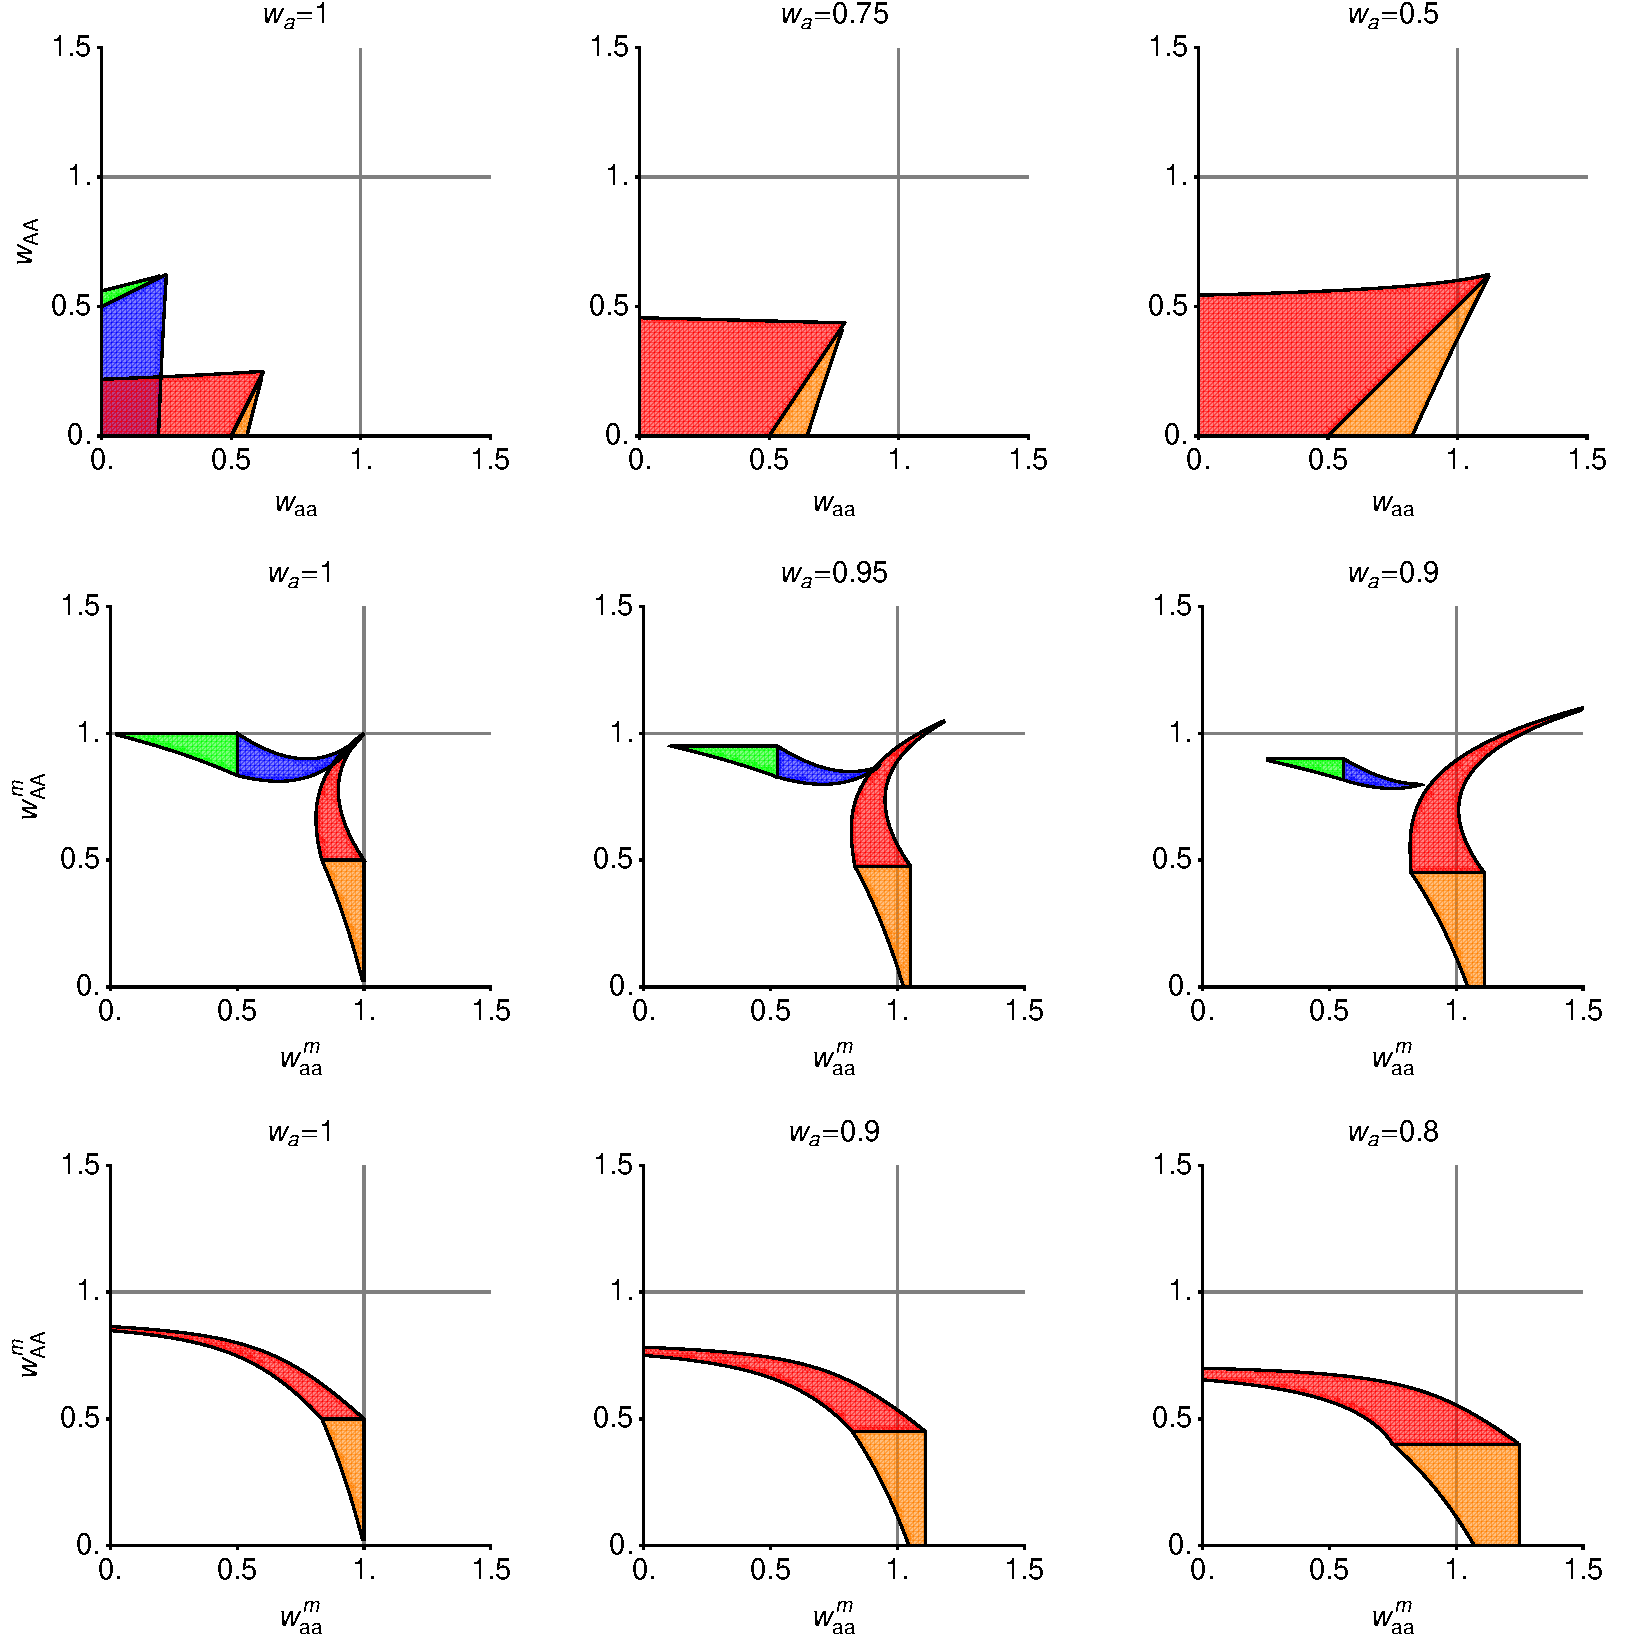
\includegraphics[width= \linewidth]{Figures/combined.pdf} 
\end{minipage}\hfill
\begin{minipage}[b]{0.25 \linewidth}
 \caption[Selection can favour increased recombination between the sex-determining region (SDR) and a selected locus that is closely linked]{
 Selection can favour increased recombination between the sex-determining region (SDR) and a selected locus that is closely linked ($r_{ij} \approx 0$), even when selection in males is not overdominant. 
 Coloured regions show where increased recombination is favoured in a population at equilibrium $(A)$ in blue, $(B)$ in green, $(A')$ in red, and $(B')$ in orange. 
 Since this model is symmetrical, red/orange regions can be exchanged with blue/green regions if the labelling of $A$ and $a$ alleles is switched. 
 Across columns we vary the fitness of $a$-bearing haploids relative to the $A$-bearing haploids ($w_{A}=1$). Grey lines show the fitness of heterozygous diploids $w_{ij}^{k}=1$.
 In the first row, there are no differences in selection between male and female diploids ($w_{ij}^{f}=w_{ij}^{m}=w_{ij}$), where $w_{aa}$ and $w_{AA}$ are varied along the x and y axes, respectively. 
 As haploid selection becomes stronger, increased recombination can evolve with weaker overdominance in diploids and also with ploidally antagonistic selection ($w_{aa}>1>w_{AA}$).
 In the second and third rows, we consider sex differences in selection, where $w_{aa}^{m}$ and $w_{AA}^{m}$ are varied along the x and y axes ($w_{Aa}^{m}=1$).
 In the second row, where selection in females is overdominant ($w_{AA}^{f}=0.75$, $w_{Aa}^{f}=1$, $w_{aa}^{f}=0.75$), increased recombination can be favoured when selection is directional (or underdominant) in males and haploid selection is moderately strong. 
 In the third row, selection favours the $A$ allele in females ($w_{AA}^{f}=1.05$, $w_{Aa}^{f}=1$, $w_{aa}^{f}=0.75$) and increased recombination can also be favoured with sexually antagonistic selection ($w_{AA}^{m}<1<w_{aa}^{m}$).
 For this plot, we assume that the modifier of recombination is unlinked ($R_{f}=R_{m}=1/2$).
}
 \label{fig:combined} 
\end{minipage}
\end{figure}




\bibliographystyle{amnatnat.bst}
\bibliography{Sex_chromosomes.bib}

%\end{article}

\end{document}
